\breaksection{Description of FutuRaM work package 2}


A full breakdown of the tasks and subtasks in WP2, along with the responsible partners is provided in \autoref{appendix:tasks}. The following sections provide a brief description of each task.

More information can be found in the grant agreement~\cite{futuram2022ga}, the consortium agreement~\cite{futuram2022ca}, the project management plan~\cite{futuram2022pmp} and the Milestone 6 report~\cite{futuram2023m6}.

\boxblue{DELIVERABLE}{\textbf{D2.1:} Report on the environmental and socioeconomic barriers to SRM recovery --- \textit{Month 47: May 2026}}

\subsection{Objectives}
WP2 will conduct foresight studies for materials critical to the EU economy, or materials that have significant impacts on EU sustainability because of their large volumes. WP2 will develop a set of coherent scenarios for material use and waste/recovery over time in various sectors in the EU: WEEE, ELV, BAT, CDW, MINW, SLASH.

\subsubsection{Context}

\textbf{Source:}~\cite{futuram2022ga}

\subsubsubsection{Modelling the future of waste generation and SRM recovery}

In WP2, modelling the foresight requires dealing with much unknown information and developments. A convincing
mathematical model on the future thus requires a strong narrative developed from stakeholders and existing literature
regarding how future circular behaviours, recycling and recovery technologies, and the overall material economy
will develop. Furthermore, if the mathematical model used is too detailed, there will be many data gaps, leading to it
being impractical to use and potentially leading to unrealistic results. This means a good balance needs to be found
between data availability and its translation into a quantification of future narratives. The narratives applied to each
scenario will follow plausible developments by taking into account stated MS policies by each regarding the material
economy (with a special emphasis on the waste and recycling stages) and optimistic outlooks of both recycling
technology using learning curves, and of increasing circular behaviour following global best practice. The rate of
development towards each of these scenarios will be used for sensitivity and uncertainty analyses, such that a measure
of the variability within each scenario is established.

\subsubsubsection{Open science}

Considering the multidisciplinary character of FutuRaM and its aim to provide consistent and robust data, procedures,
models, and methods, a critical discussion, harmonisation and integration of the concepts, perspectives and is crucial
for the success of the project. 


The consortium is committed to making the data available in open formats during the project and free of charge for
the EC and all stakeholders to use and publish, along with other relevant reports tailored for the use of the EC and
respecting FutuRaM’s open science principles. 


\subsubsubsection{Gender}
Within the FutuRaM, project no specific population group will be targeted. In contrast, the consortium is aware that
research often has a diversity problem since many groups are underrepresented, e.g. women, ethnic minorities, people
with disabilities and socially disadvantaged populations and we will consider specific measures that will help to
address specifically these groups. 

We will especially consider the involvement of a variety of stakeholders in WP7. 

In work packages 2, 3 and 5 we will use Delphi panels, which have an equal representation of gender and an appropriate age distribution that encapsulates multiple perspectives. In the modelling of WP2 and 4 (foresight and stock and flow models), consumption of household electronics may increase with increasing gender equality, and behavioural aspects of waste separation which could be an aspect of foresight of stock and flows. 

\section{Task Descriptions}
\begin{enumerate}[label=Task 2.\arabic*., style=nextline]
    \item \textbf{Develop scenario storyline (ULEI, TUB, Empa, Chalmers, WEEE Forum, BRGM, UNITAR, SGU) (M01-M18):}
    This task involves scanning, mapping, and assessing scenarios used in the grey, scientific, policy, and industry literature/reporting for the different waste streams, (e.g., the Shared Socioeconomic Pathways, the International Resource Panel Scenarios, the International Energy Agency Scenarios, etc) to develop cogent storylines for the three planned scenarios. These will cut across sectors and will be used for the Stock-Flow models (WP4) and will include the translation of general concepts such as stated policies, sustainable development, circular economy, to each sector. FutuRaM will develop at minimum three scenarios (1. Sustainability, 2. Recoverability, and 3. Business-as-usual).

    \item \textbf{Integrate future technologies into the scenarios (Chalmers, ULEI, TUB, Empa, WEEE Forum, BRGM, UNITAR, UCL, LMU, SGU, VITO) (M03-M20):}
    This task will review current and emerging technologies used in the various sectors for product manufacturing and end-of-life handling, with a special emphasis on material production, use, and recycling. Together with the storylines developed in Task 2.1, it will adapt the market share of these technologies for each sector to determine the future development of each sector.

    \item \textbf{Forecast material composition and products for each scenario (TUB, ULEI, UNITAR, Chalmers, BRGM, Empa, VITO) (M7-M20):}
    Following the scenarios from T2.1, the material compositions and future products for each sector will be determined based on the product and commodity demand and technology realisation (T2.2). This task will be coupled to the data collection in WP3 and WP4.

    \item \textbf{Quantify environmental and socioeconomic impacts of SRM recovery under each scenario (ULEI, TUB, Empa, UNITAR, WEEE Forum, BRGM, UCL, LMU) (M18-M36):}
    This task will use the information generated in Tasks 2.1-2.3, together with the material flow analysis from WP4, to quantify the future environmental and socioeconomic feedbacks for each waste sector and scenario according to future recovery technology.

    \item \textbf{Assess the environmental and socioeconomic impacts and bottlenecks of future SRM recovery (ULEI, TUB, Empa, UNITAR, Chalmers, UNITAR. WEEECycling) (M37-M47):}
    This task will develop a report based on an assessment on the pressures and bottlenecks associated with environmental and socioeconomic issues related to each waste sector, including the associated changes and impacts on imports and of primary raw materials production (D2.1).
\end{enumerate}

\begin{landscape}
\subsection{Interconnection with other work packages in FutuRaM}

\boxreview{Does anyone have the original, editable version of this figure?} 

\autoref{fig:wp2_interconnection} shows the interconnection between WP2 and the other work packages in FutuRaM~\cite{futuram2022ga}.

\begin{figure}[ht!]


    \vspace{1cm}
    \centering
    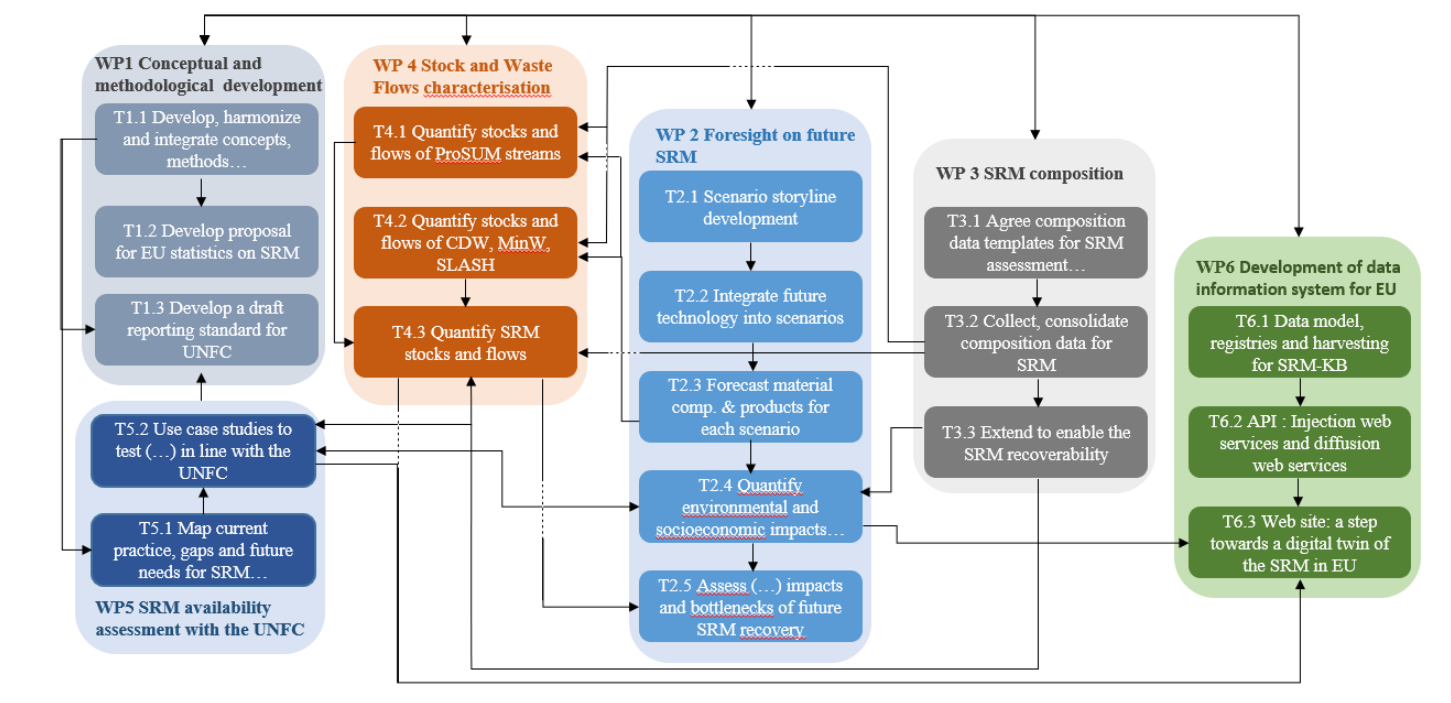
\includegraphics[width=\linewidth]{000frontmatter/wp2_interconnections.png}
    \caption{Interconnection between WP2 and the other work packages in FutuRaM}
    \label{fig:wp2_interconnection}
\end{figure}
\end{landscape}

\begin{landscape}
        \subsection{Work package two milestones}
        \small
        \centering
        \noindent
        \begin{table}[ht!]
        \caption{WP2.1 --- Milestone list}\label{tab:milestones}
        \begin{tabular}{|L{1cm}|L{7cm}|L{1cm}|L{2cm}|L{3cm}|L{9cm}|}
        \arrayrulecolor{headerblue}\hline
        \rowcolor{headerblue}\color{white}\textbf{M\#} & \color{white}\textbf{MILESTONE NAME} & \color{white}\textbf{WP} & \color{white}\textbf{DUE DATE} & \color{white}\textbf{RESP. PARTNER} & \color{white}\textbf{MEANS OF VERIFICATION} \\
        \arrayrulecolor{black}\hline
        MS11 & Mapping of published scenarios and Storyline/scenario description & 2 & Dec. 2023 & ULEI & Datasets on available scenarios are fed into D1.1 and qualitative descriptions of 3 futures for the six waste streams are circulated \\
        \hline
        MS17 & Mapping of future technologies for each sector & 2 & Feb. 2024 & ULEI & Dataset covering sector-specific current and emerging technologies in both the production of products and their end-of-life treatment made available to WP1 Lead and consortium members, including quantitative descriptions of future product market shares related to 6 waste streams \\
        \hline
        MS20 & Integration of social, environmental, and economic assessments & 2 & May 2026 & ULEI & Social, environmental, and economic impacts of SRM recovery have been quantified for each scenario and waste stream. Information delivered to the consortium. \\
        \hline
        \end{tabular}
        \end{table}
\end{landscape}

\begin{landscape}
        \subsection{Subtasks for Task 2.1 --- Scenario storyline development}
        \noindent
        \begin{table}[ht!]
        \caption{WP2.1 --- Subtask list}\label{tab:subtasks-2.1}
        \centering
        \rowcolors{2}{white}{fadedblue} % Alternate colors starting from row 2
        \begin{tabular}{|L{0.5cm}|L{1cm}|L{1.5cm}|L{2cm}|L{2cm}|L{7cm}|L{1cm}|L{1cm}|L{4cm}|L{1.5cm}|}
        \arrayrulecolor{headerblue}\hline
        \rowcolor{headerblue}\color{white}\textbf{WP} & \color{white}\textbf{TASK} & \color{white}\textbf{SUB-TASK} & \color{white}\textbf{NAME} & \color{white}\textbf{WS} & \color{white}\textbf{DESCRIPTION} & \color{white}\textbf{START} & \color{white}\textbf{END} & \color{white}\textbf{PARTNERS} & \color{white}\textbf{STATUS} \\
        \arrayrulecolor{black}\hline
        2 & 2.1 & 2.1 & Scenario mapping & Cross-cutting & Map various studies from the academic, policy, and grey literature for future scenarios and assess the applicability within FutuRaM & M01 & M05 & WEEE Forum, UNITAR, BRGM, CU, GTK, LMU, RECHARGE, SGU, TUB, LU, VITO, Empa, UCL & \checkmark \\
        \hline
        2 & 2.1 & 2.2 & Scenario methods & Cross-cutting & Compile various methodologies for scenario development and assess their applicability for developing scenarios on material recovery and circular economy for Europe & M02 & M05 & WEEE Forum, UNITAR, BRGM, CU, GTK, LMU, RECHARGE, SGU, TUB, LU, VITO, Empa, UCL & \checkmark \\
        \hline
        2 & 2.1 & 2.3 & Scenario storylines & Cross-cutting & Flesh out the storylines of the 3 main scenarios & M05 & M08 & UNITAR, CU, TUB, LU & \checkmark \\
        \hline
        2 & 2.1 & 2.4 & Qualitative scenario development & Cross-cutting & Use the chosen methods and qualitative methods to develop the three main scenarios to be used in FutuRaM (e.g. BAU, increased material recovery, and full circular economy) & M07 & M11 & UNITAR, CU, SGU, LU, VITO, UCL & \checkmark (V3) \\
        \hline
        \end{tabular}
        \end{table}
\end{landscape}

\begin{landscape}
    \subsection{Consortium partner contributions to WP2}
    \autoref{tab:wp2_personmonths} lists the consortium partner contributions to WP2, in terms of person months for each sub-task. The table is based on the FutuRaM grant agreement~\cite{futuram2022ga}.
    \begin{table}[h!]
        \centering
        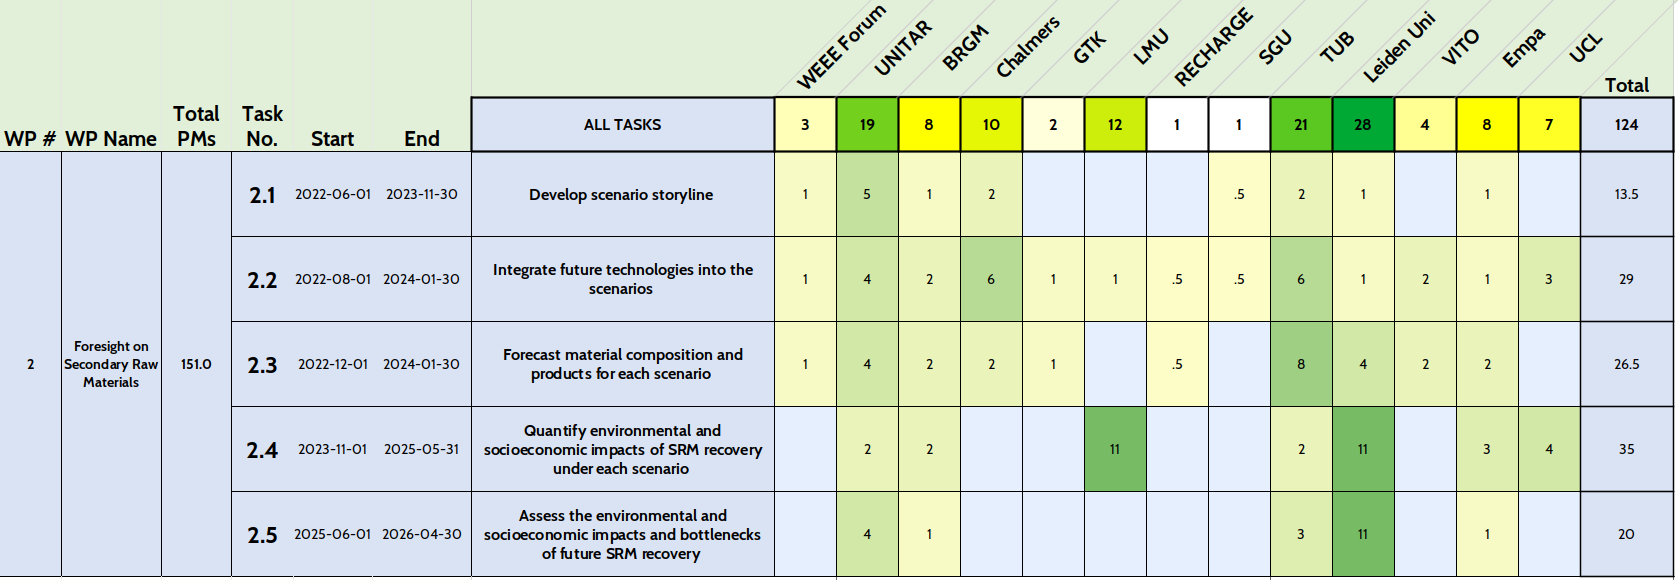
\includegraphics[width=\linewidth]{000frontmatter/wp2_personmonths.png}
        \caption{Consortium partner contributions to WP2 (person months per sub-task)}\label{tab:wp2_personmonths}
    \end{table}
\end{landscape}

\clearpage

